\documentclass{article}
\usepackage[utf8]{inputenc}
\usepackage{blindtext}
\usepackage{graphicx}
\usepackage{amsmath}
\usepackage{csvsimple}
\usepackage{pdfpages}
\usepackage{hyperref}
\usepackage{caption}
\usepackage{subcaption}

\title{Kapitán Brown}
\author{Martin Skok}

\begin{document}
\maketitle

\begin{abstract}
  Opilý kapitán Brown jde z hospody v 1D rovině (nikdy jsem nepsal abstrakt)
\end{abstract}

\section{Zadání}
Kapitán Brown vyjde v čase t = 0 z hospody v x = 0 a v každém kroku se s
pravděpodobností ½ přemístí o jeden krok vlevo nebo vpravo.
Zvolte vhodnou délku procházky tmax a počet opakování N pro získání statisticky
spolehlivých výsledků.\\
\newpage
\section{Data}
Jako první jsem nasimuloval náhodnou procházku v 1D. Použil jsem $t_{max} = 1000$
a $N = 1000$, kde $t_{max}$ je vlastně čas neboli dékla procházky a $N$ je počet procházek celkem.
Protože se data zdála nedostatečná, navýšil jsem počet opakování na $N = 10000$

\begin{figure}[hbt!]
  \begin{center}
    \includegraphics[scale=0.7]{walks.pdf}
    \end{center}
  \caption{Simulace náhodných procházek}
\end{figure}
\newpage

Poté jsem měl určit křivku $<x^{2} (t)>$.
Určil jsem ji tak, že jsem udělal průměr všech křivek na druhou mocninu.

\begin{figure}[hbt!]
  \begin{center}
    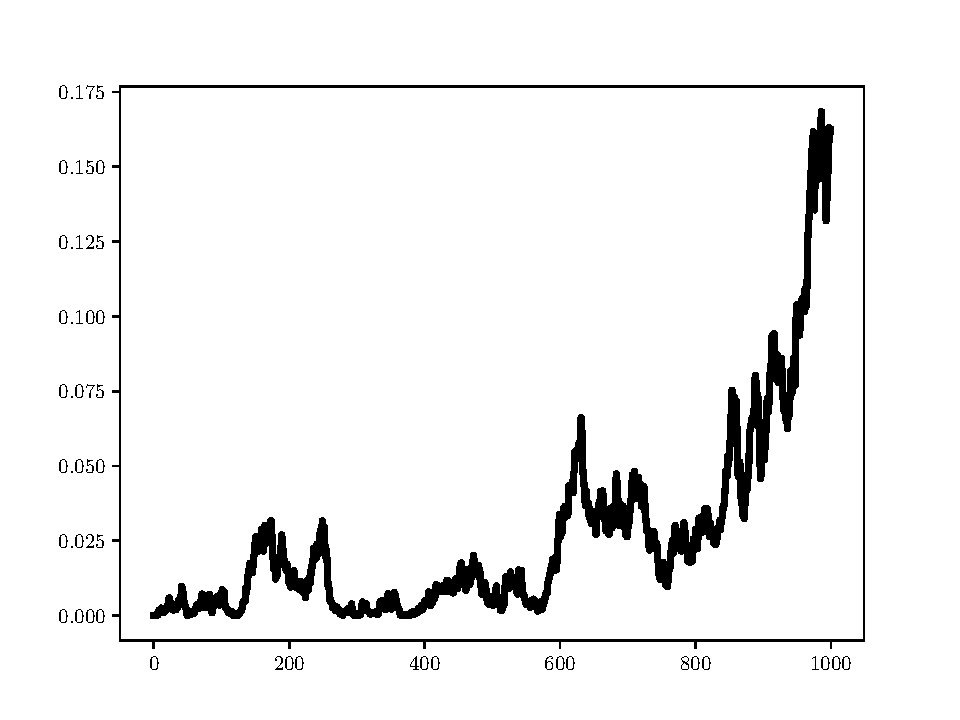
\includegraphics[scale=0.7]{walks2.pdf}
    \end{center}
  \caption{Křivka $<x^{2} (t)>$}
\end{figure}


\newpage
\section{Data}
Dále jsem si měl vybrat různé časové intervali a udělat v těchto časech historogramy.
Vybral jsem tedy 12 náhodných intervalů mezi $t_{i} \in [300, 10000]$.\\
Historogramy jsem nemusel normovat manuálně, program to udělal za mě, jak je popsáno v kodu.
$\sigma$ a $\mu$ program našel za mě taky.

\begin{figure}
\begin{subfigure}{.3\textwidth}
  \centering
  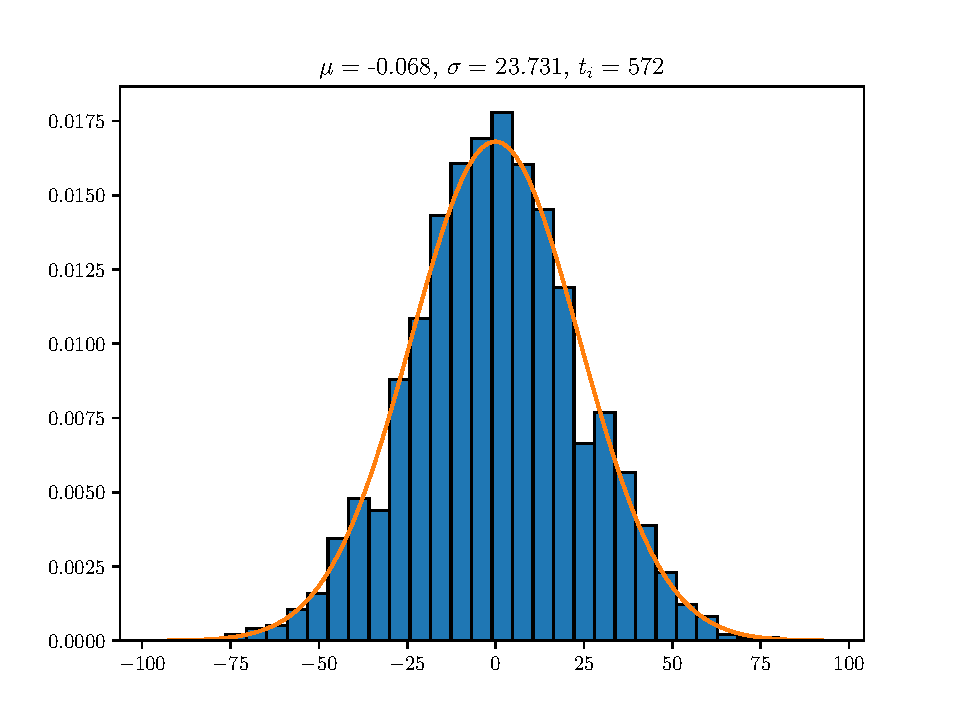
\includegraphics[width=1.1\linewidth]{hist1.pdf}
\end{subfigure}
\begin{subfigure}{.3\textwidth}
  \centering
  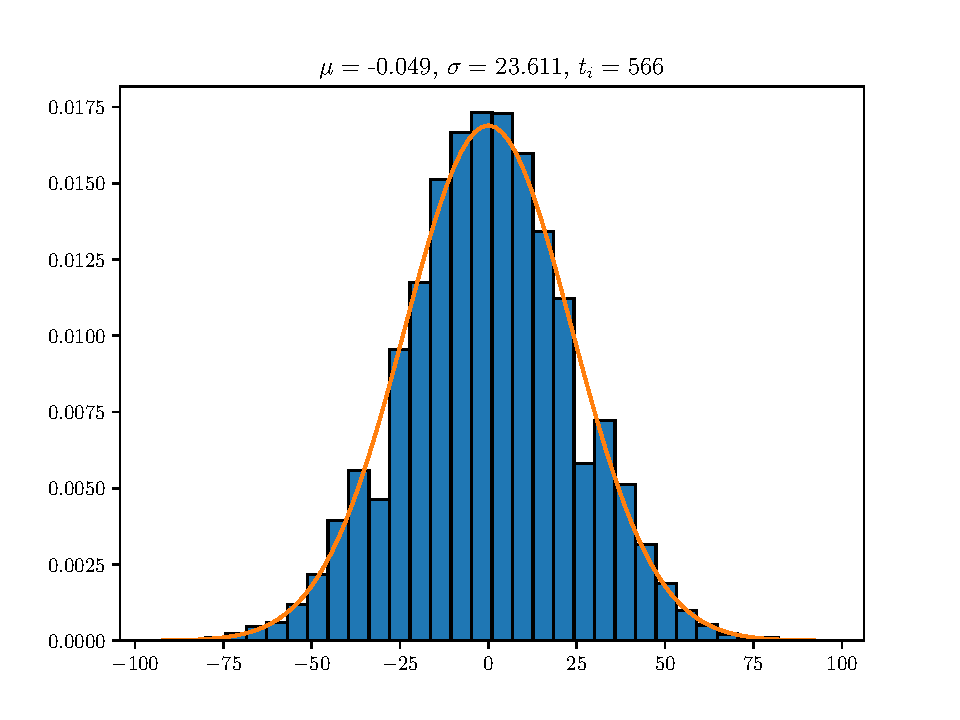
\includegraphics[width=1.1\linewidth]{hist2.pdf}
\end{subfigure}
\begin{subfigure}{.3\textwidth}
  \centering
  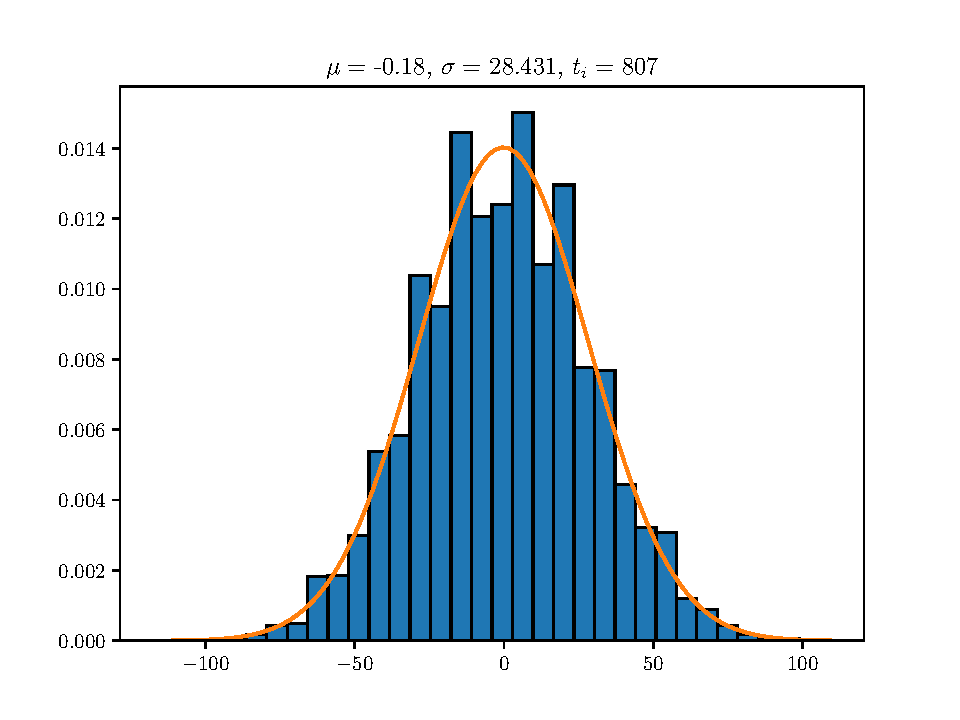
\includegraphics[width=1.1\linewidth]{hist3.pdf}
\end{subfigure}
\newline

\begin{subfigure}{.3\textwidth}
  \centering
  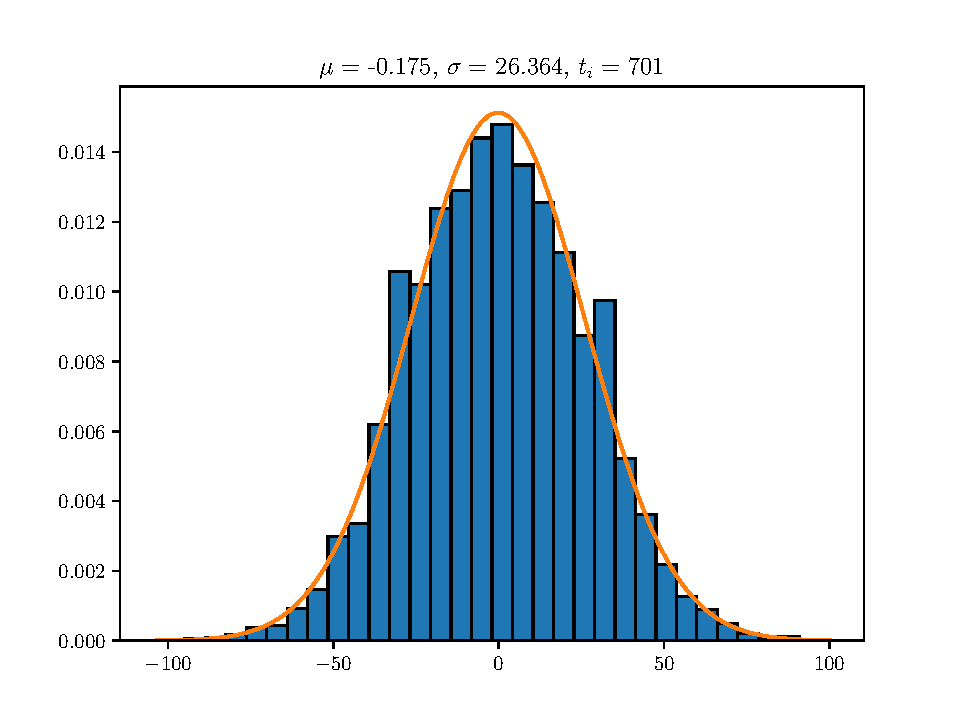
\includegraphics[width=1.1\linewidth]{hist4.pdf}
\end{subfigure}
\begin{subfigure}{.3\textwidth}
  \centering
  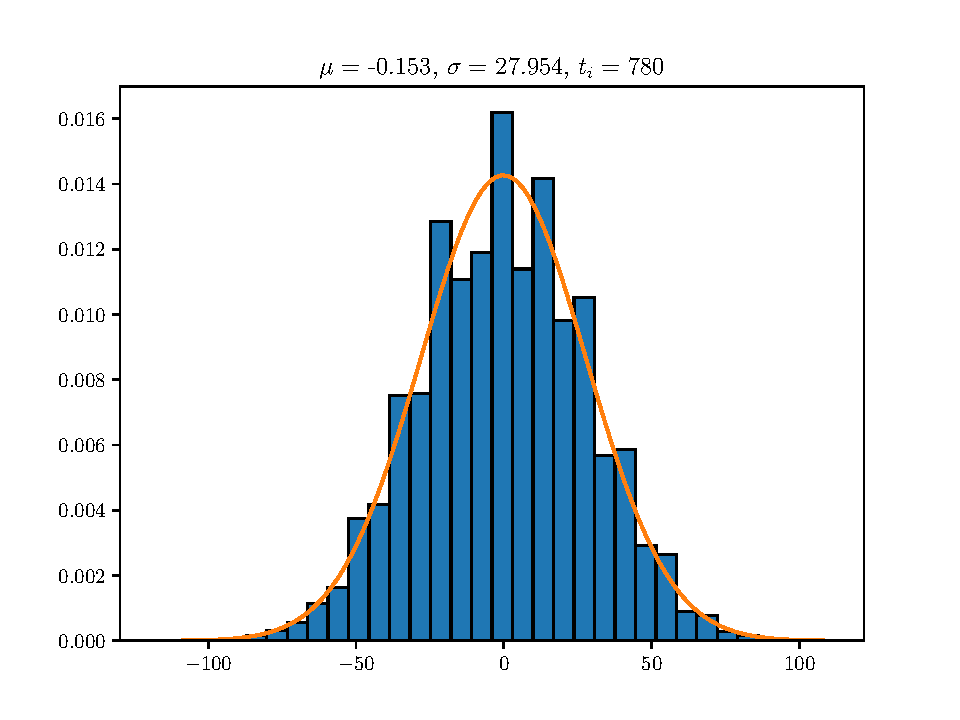
\includegraphics[width=1.1\linewidth]{hist5.pdf}
\end{subfigure}
\begin{subfigure}{.3\textwidth}
  \centering
  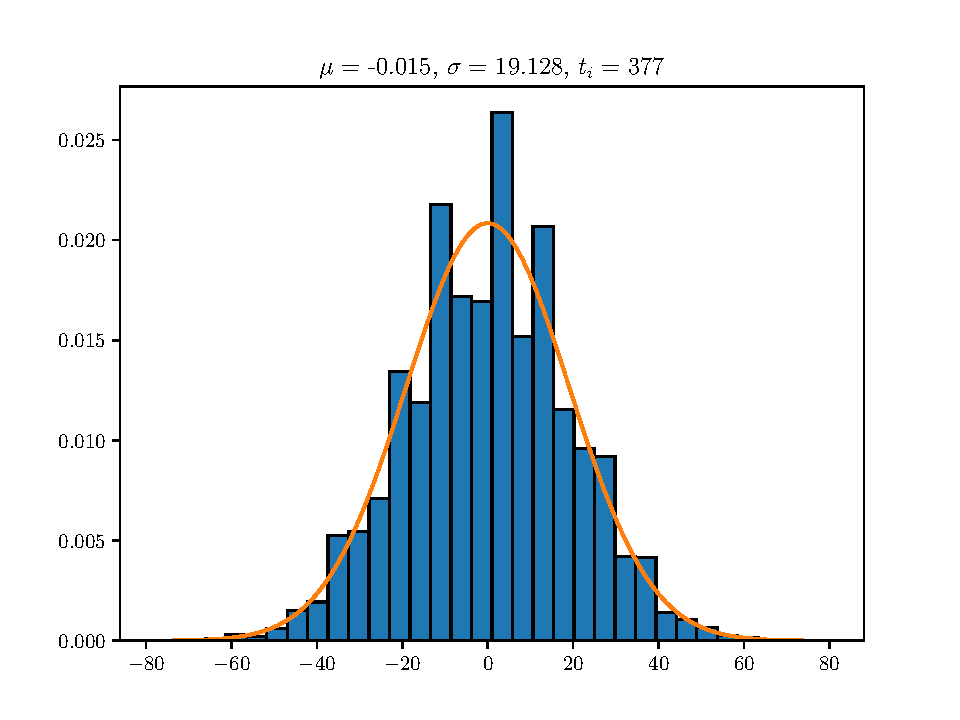
\includegraphics[width=1.1\linewidth]{hist6.pdf}
\end{subfigure}
\newline

\begin{subfigure}{.3\textwidth}
  \centering
  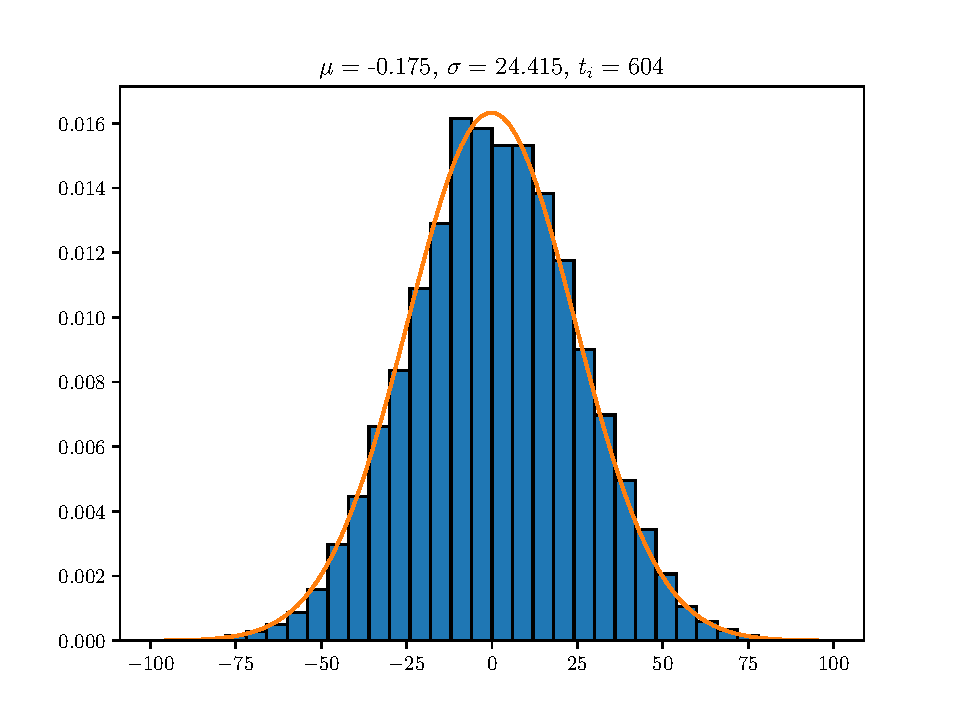
\includegraphics[width=1.1\linewidth]{hist7.pdf}
\end{subfigure}
\begin{subfigure}{.3\textwidth}
  \centering
  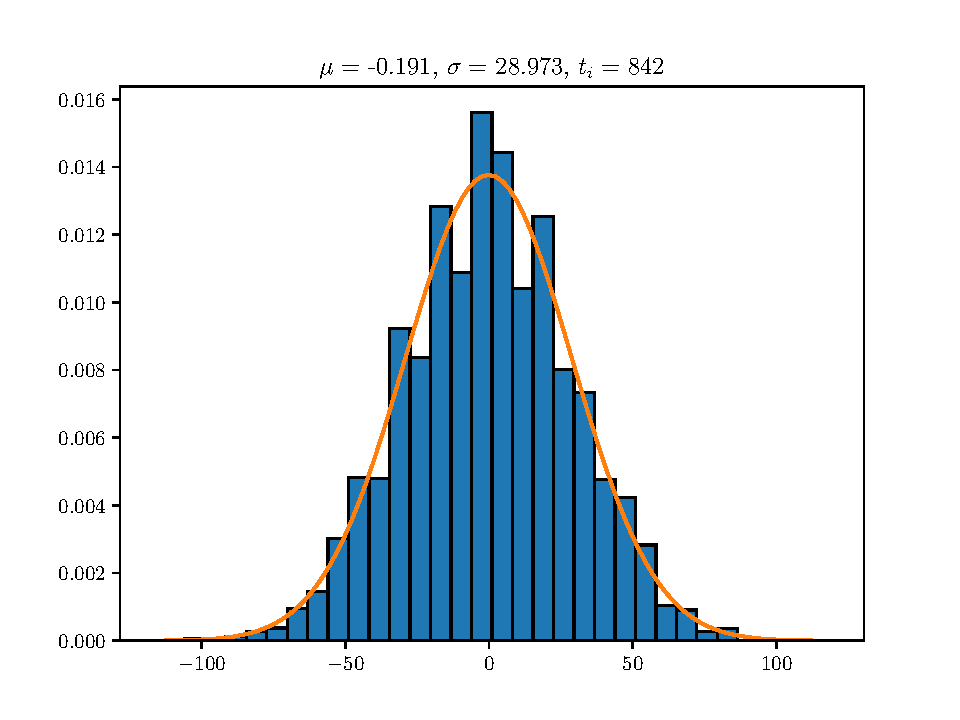
\includegraphics[width=1.1\linewidth]{hist8.pdf}
\end{subfigure}
\begin{subfigure}{.3\textwidth}
  \centering
  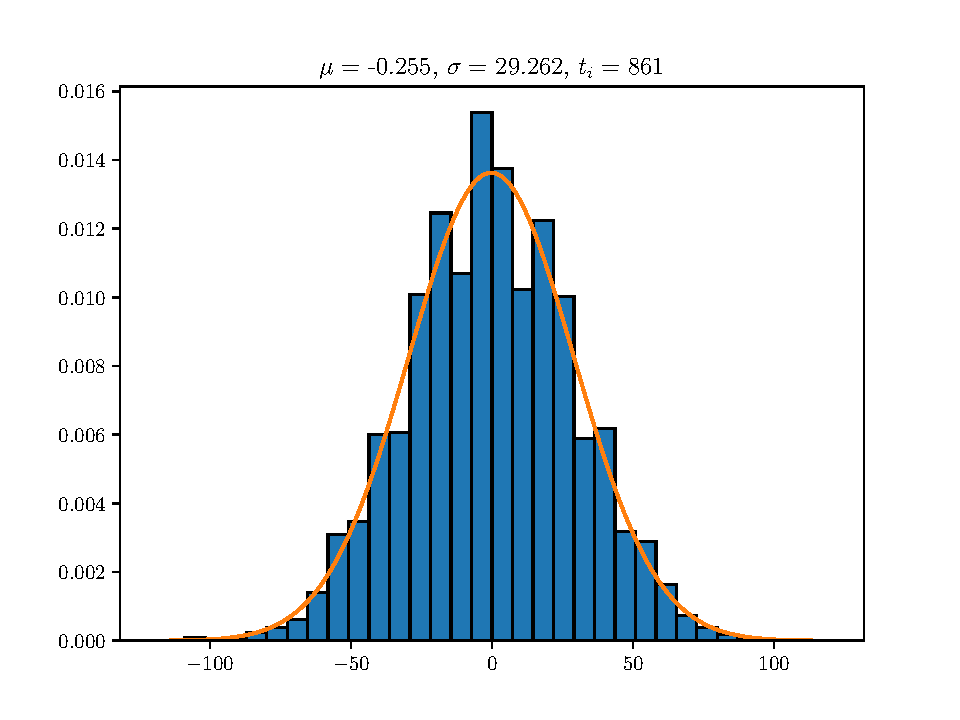
\includegraphics[width=1.1\linewidth]{hist9.pdf}
\end{subfigure}
\newline

\begin{subfigure}{.3\textwidth}
  \centering
  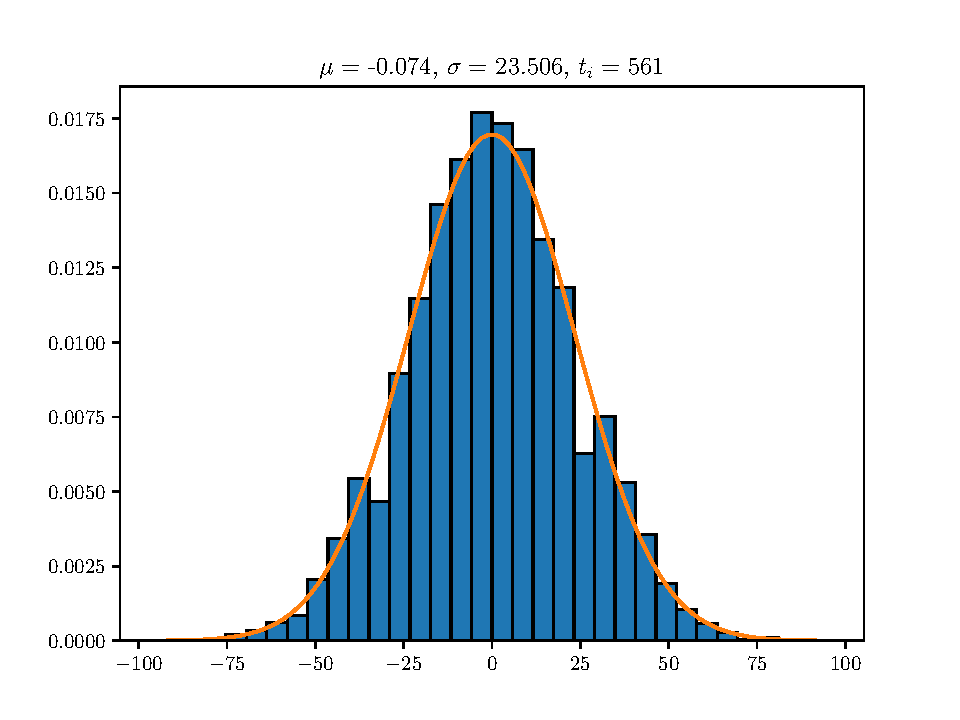
\includegraphics[width=1.1\linewidth]{hist10.pdf}
\end{subfigure}
\begin{subfigure}{.3\textwidth}
  \centering
  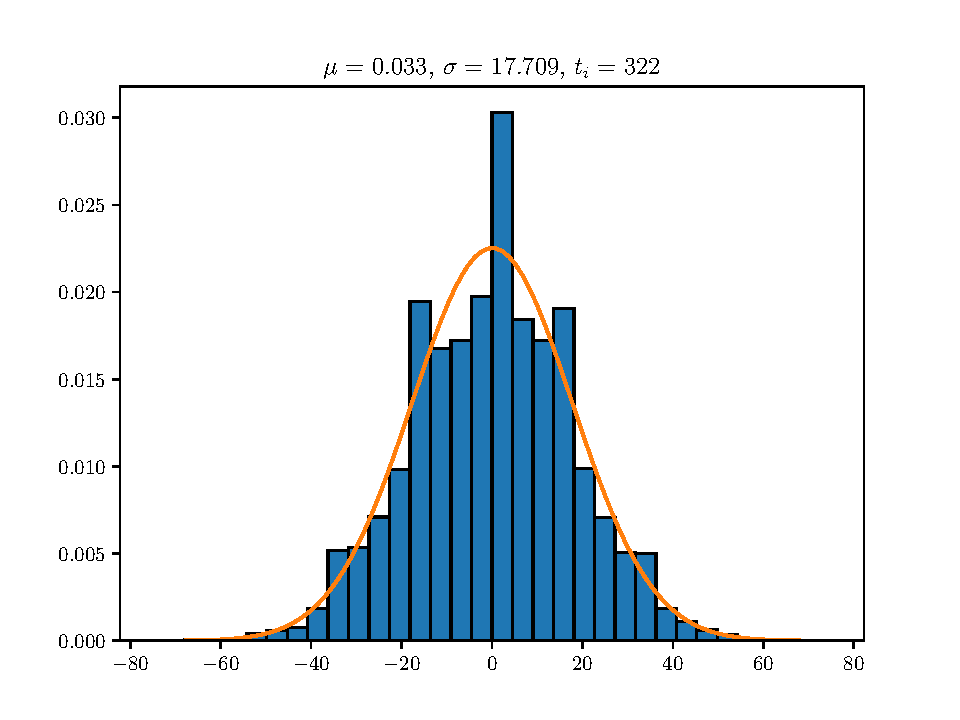
\includegraphics[width=1.1\linewidth]{hist11.pdf}
\end{subfigure}
\begin{subfigure}{.3\textwidth}
  \centering
  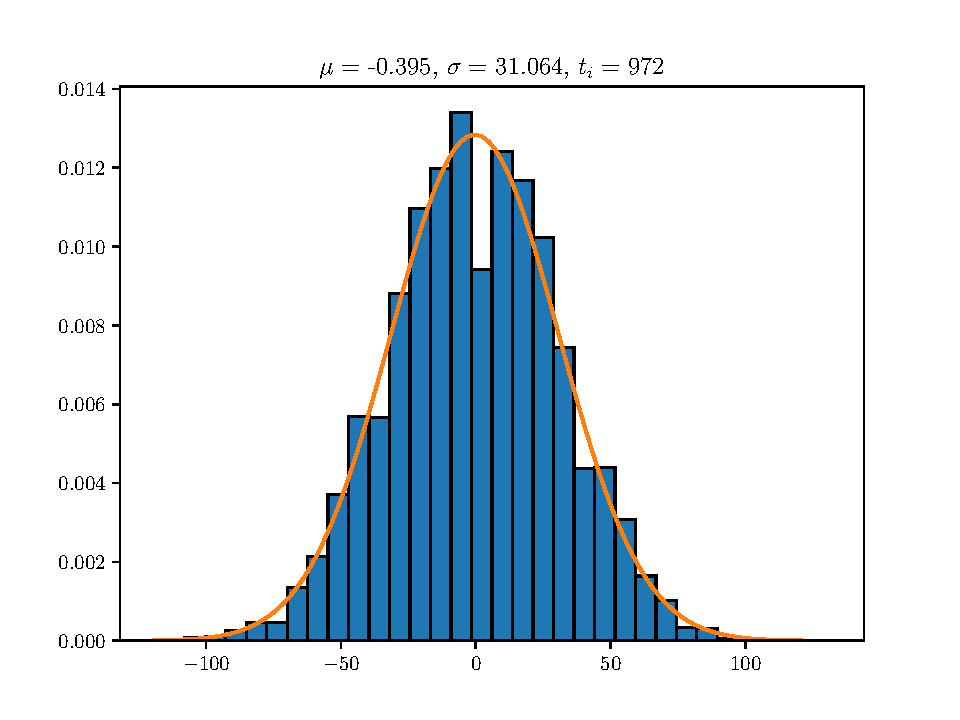
\includegraphics[width=1.1\linewidth]{hist12.pdf}
\end{subfigure}
\newline

\caption{Historogramy}
\end{figure}

\newpage
Abych určil závislost $\sigma$ na $t_{i}$, vytvořil jsem tabulku.
Tabulka není řádně seřazena, protože jsem hodnoty generoval náhodně,
takže líp je to vidět až na grafu.
  \begin{table}[!ht]
    \centering
    \begin{tabular}{|l|l|l|}
    \hline
        time & mu & sigma \\ \hline
        755.0 & -0.109 & 27.459 \\ \hline
        572.0 & -0.068 & 23.731 \\ \hline
        566.0 & -0.049 & 23.611 \\ \hline
        807.0 & -0.18 & 28.431 \\ \hline
        701.0 & -0.175 & 26.364 \\ \hline
        780.0 & -0.153 & 27.954 \\ \hline
        377.0 & -0.015 & 19.128 \\ \hline
        604.0 & -0.175 & 24.415 \\ \hline
        842.0 & -0.191 & 28.973 \\ \hline
        861.0 & -0.255 & 29.262 \\ \hline
        561.0 & -0.074 & 23.506 \\ \hline
        322.0 & 0.033 & 17.709 \\ \hline
        972.0 & -0.395 & 31.064 \\ \hline
        654.0 & -0.182 & 25.501 \\ \hline
        707.0 & -0.217 & 26.502 \\ \hline
        498.0 & -0.071 & 22.009 \\ \hline
        908.0 & -0.261 & 30.061 \\ \hline
        533.0 & -0.109 & 22.857 \\ \hline
    \end{tabular}
    \caption{Tabulka ukazující závistlost $t_{i}$ a $\sigma$}
  \end{table}
  \\
  Z tabulky není moc vidět, že čím větší je čas $t_{i}$, tím je větší i $\sigma$, ale je to tak.\\
  \newpage
  Z grafu je vidět, že tato závislost $\sigma(t_{i})$ není lineární i když se to
  na první pohled může zdát. Na grafu je zobrazena pomocí modrých teček.
  Tyto data jsou fitnuty křivkou, která je na grafu zobrazena pomocí
  modré čáry a je popsána rovnicí:
  $$f(t) = 1.1 \cdot t_{i}^{0.49} - 1.12$$

\begin{figure}[hbt!]
  \begin{center}
    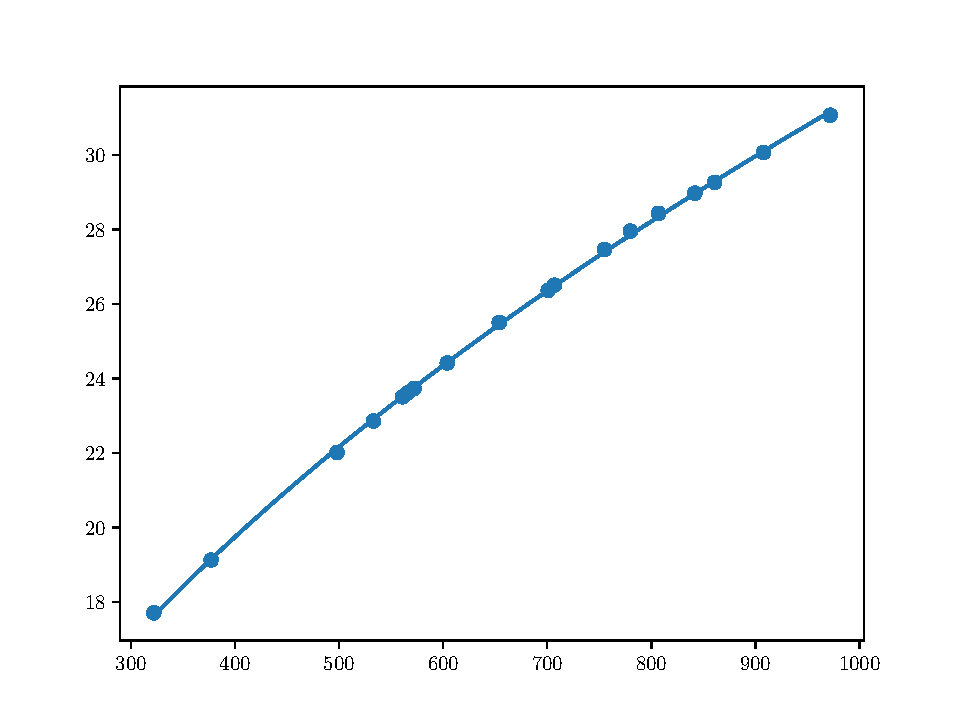
\includegraphics[scale=0.7]{lin.pdf}
    \end{center}
  \caption{Graf ukazující závistlost $t_{i}$ a $\sigma$}
\end{figure}
\newpage

\end{document}
